%%%%%%%%%%%%%%%%
\section{Control Solution}
\begin{frame}{Control Solution}{}
    \centering
    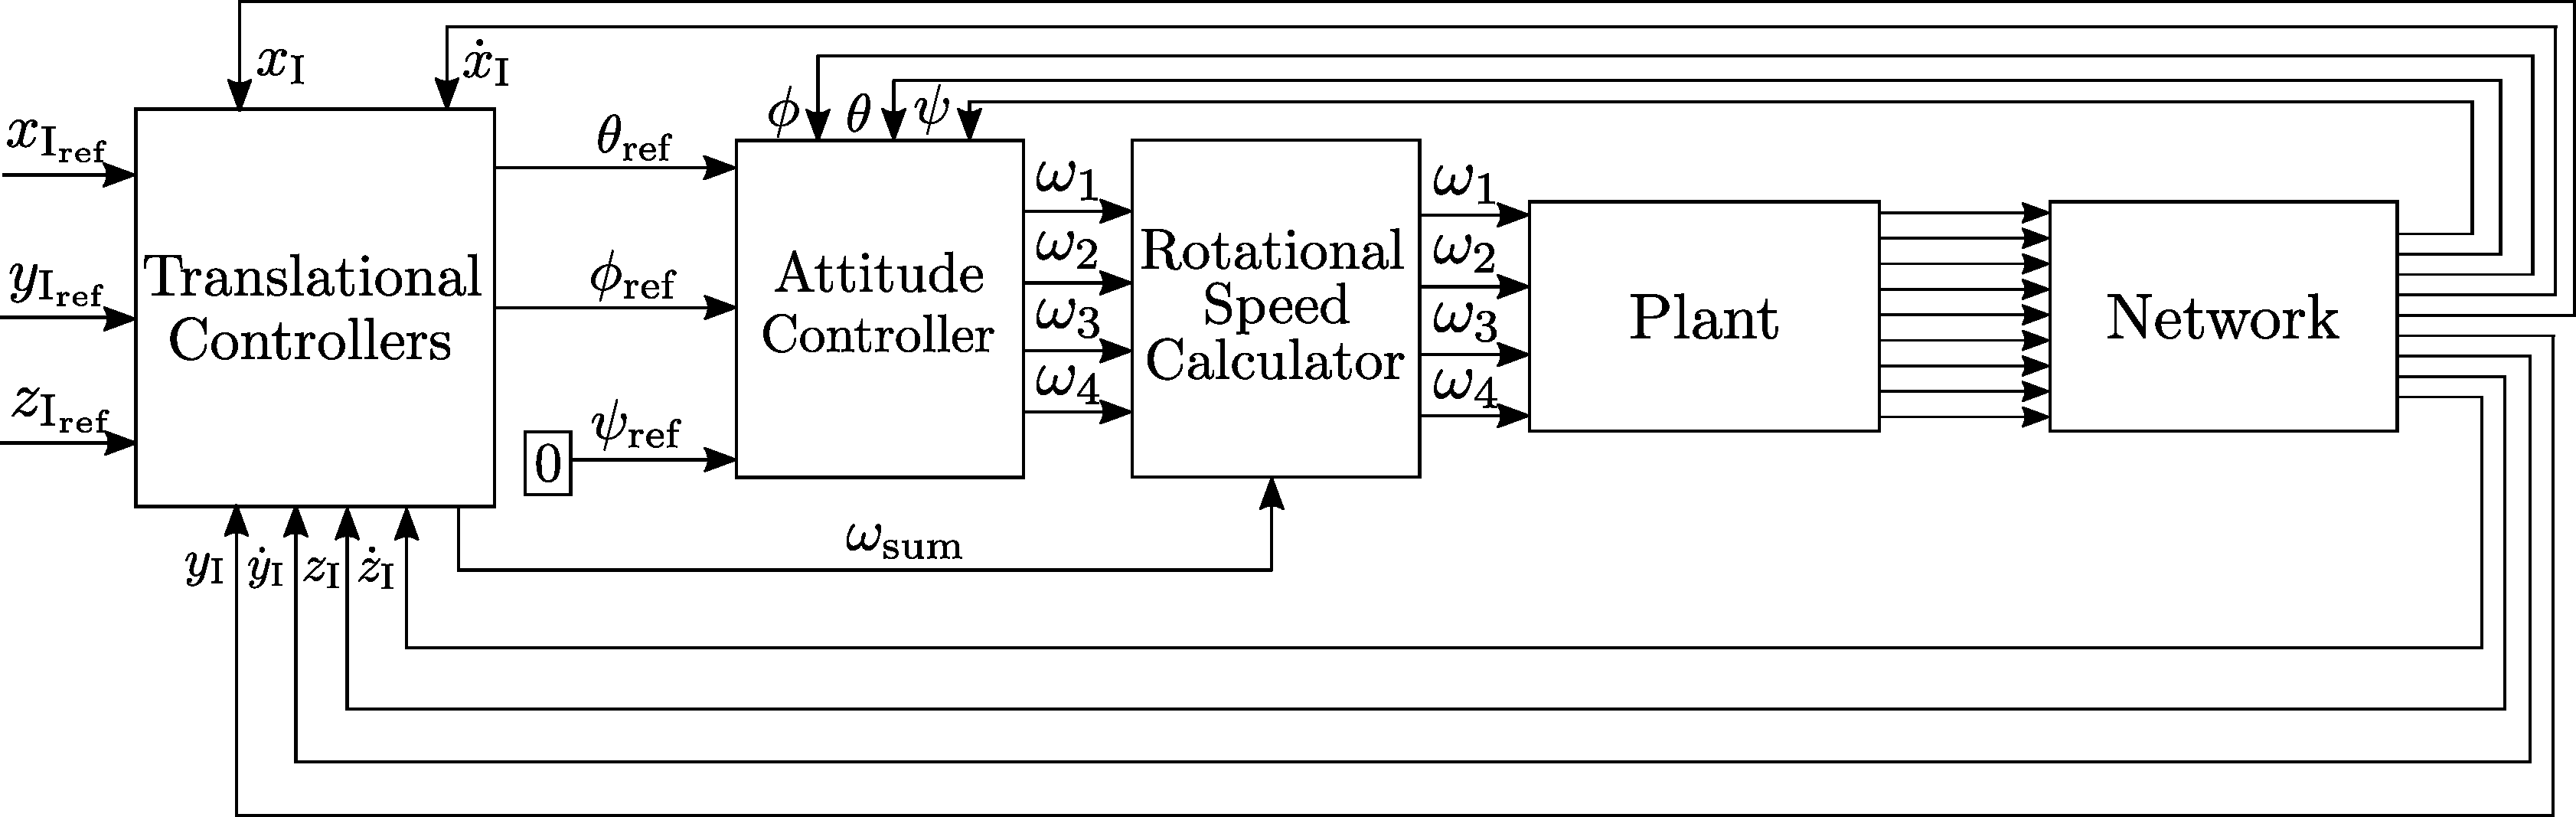
\includegraphics[scale=0.2]{figures/ControlDiagramPoster}
\end{frame}

\subsection{Attitude Controller}
\begin{frame}{Control Solution}{Attitude Controller}
    \centering
    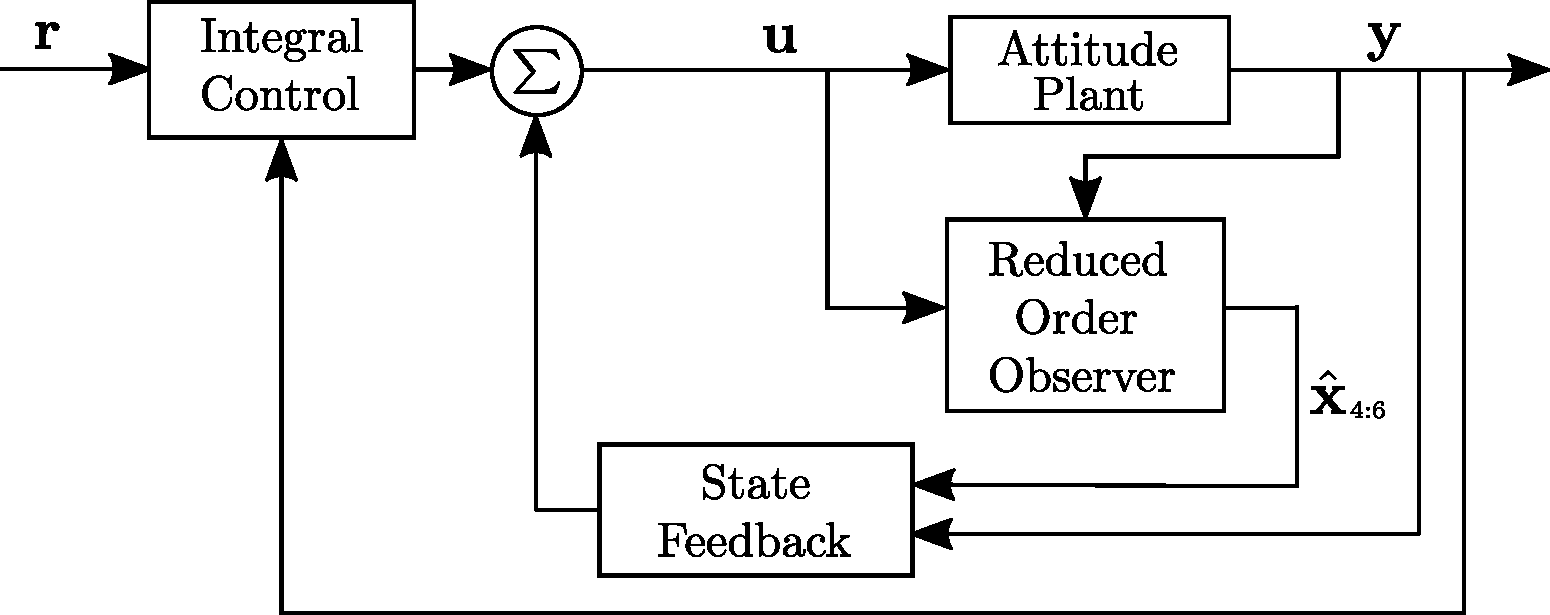
\includegraphics[scale=0.35]{figures/AttitudeControlDiagram}    
\end{frame}

\begin{frame}{Control Solution}{Attitude Controller}
    \begin{itemize}
        \item System Representation
    \end{itemize}

%    \begin{figure}
%        \begin{tikzpicture}[ auto,
                       thick,                         %<--setting line style
                       node distance=1.5cm,             %<--setting default node distance
                       scale=1,                     %<--|these two scale the whole thing
                       every node/.style={scale=1}, %<  |(always change both)
                       >=triangle 45 ]                %<--sets the arrowtype
    
    \draw%-----------------------------------------------------------------------------------------
    	%Drawing Input/Output:
    	node[shape=coordinate][](input1) at (0,0){}
    	node[shape=coordinate][](output1) at (9.5,0){}
     	%Drawing the Equation Blocks:   	
      	node(A) at (4.5,-1.5) [block] {A} 
     	node(B) at (1.5,0) [block] {B}
     	node(C) at (6.5,0) [block] {C}
      	node(D) at (4.5,1.5) [block] {D}  
	    node(int) at (4.5,0) [block] {\si{\int}}  
    	%Drawing the Sumation Blocks:	    	 	
    	node(sum1) [sum, right of = B] {\si{\sum}}
    	node(sum2) [sum, right of = C] {\si{\sum}}
    	%Drawing the Feedback/Feedforward Nodes:    	
    	node[shape=coordinate][](FeedforwardNode) at (0.75,0){}
    	node[shape=coordinate][](FeedbackNode) at (5.5,0){}  	
    	     
    ;%---------------------------------------------------------------------------------------------
   
    %Joining the Blocks
  	\draw[->](input1) -- node {u}(B);
  	\draw[->](B) -- node {}(sum1);
  	\draw[->](sum1) -- node {\si{\dot x}}(int);  	
  	\draw[->](int) -- node {x}(C);
  	\draw[->](C) -- node {}(sum2);  	
  	\draw[->](sum2) -- node {y}(output1);
  	
  	\draw[->](FeedforwardNode) |- node{} (D);
  	\draw[->](D) -| node{} (sum2);

  	\draw[-] (FeedbackNode) |- (A);
  	\draw[->] (A)   -| (sum1);

    %Drawing node(s) with \textbullet
    \draw%--------------------------------------------------------------
      node at (input1)  [shift={(-0.08, -0.02 )}] {\large \textbullet}
    	% node at (output1) [shift={( 0.008, -0.02 )}] {\textbullet}
    ;%------------------------------------------------------------------
  \end{tikzpicture}
%    \end{figure}
\end{frame}


\begin{frame}{Control Solution}{Attitude Controller}
    \begin{itemize}
        \item State Feedback with Integral Control
    \end{itemize}
    
    \centering
%    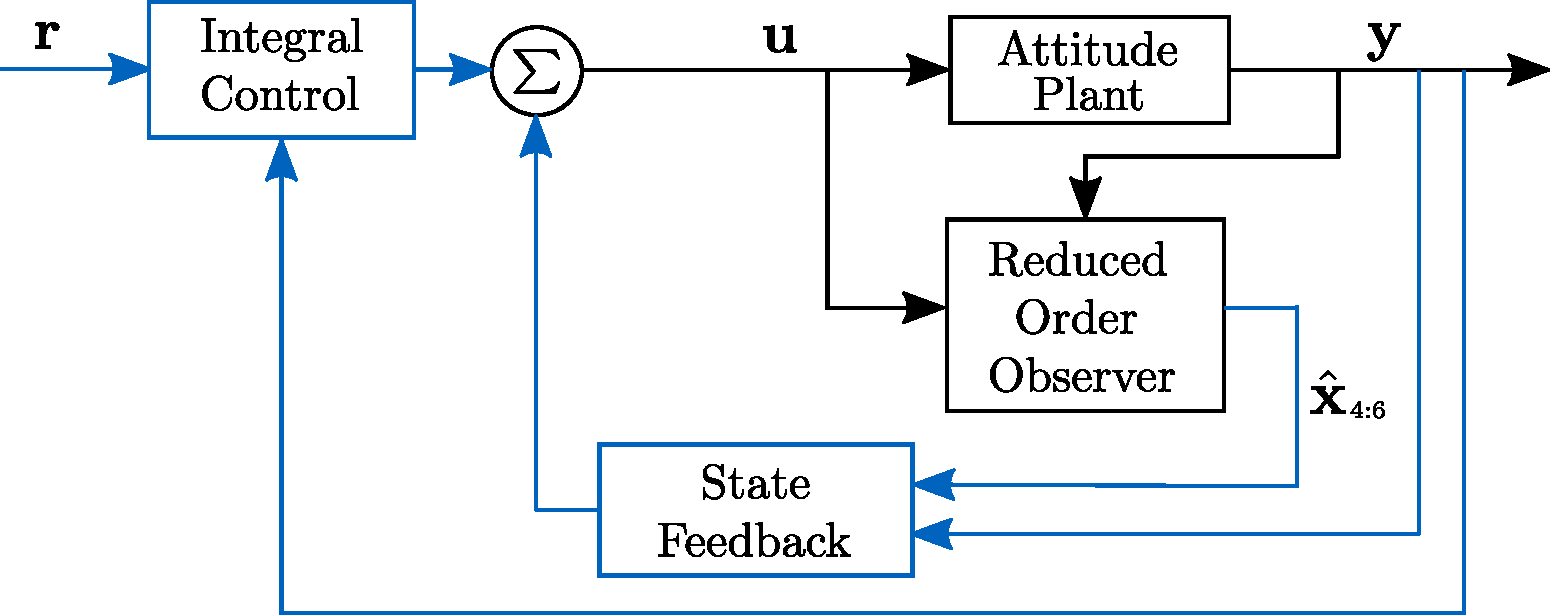
\includegraphics[scale=0.25]{figures/ControllerColorDiagram}  \\
%    \vspace{1cm}
    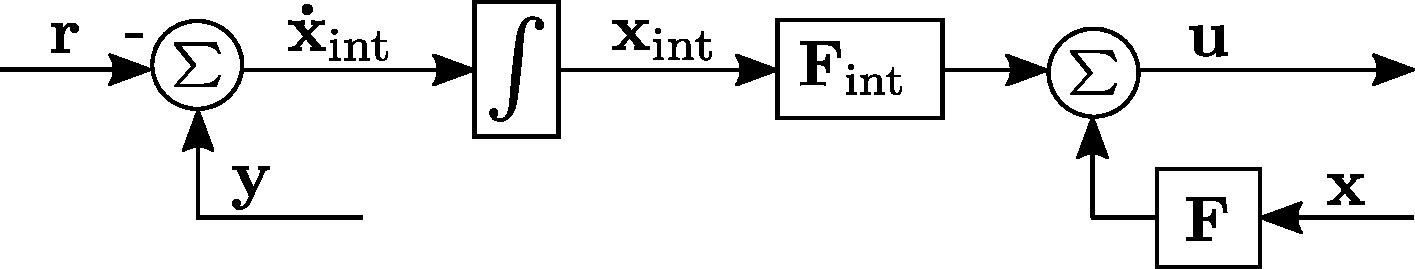
\includegraphics[scale=0.35]{figures/DetailedControllerColorDiagram}  
    
    extended
\end{frame}

\begin{frame}{Control Solution}{Attitude Controller}
    \begin{itemize}
        \item LQR
    \end{itemize}
    \begin{flalign} 
        J &= \int_{0}^{\infty} \vec{x}^T \vec{Q} \vec{x} + \vec{u}^T \vec{R} \vec{u} \ dt \nonumber
    \end{flalign}
     \begin{itemize}
         \item Bryson's Rule
     \end{itemize}   
    \begin{flalign} 
    Q_{ii} &= \frac{1}{\text{maximum acceptable value of }[x^2_i]}\nonumber\\
    R_{ii} &= \frac{1}{\text{maximum acceptable value of }[u^2_i]}\nonumber
    \end{flalign}
    
\end{frame}

\begin{frame}{Control Solution}{Attitude Controller}
    \begin{itemize}
        \item Reduced Order Observer
    \end{itemize}
%
%
%    \begin{minipage}{\linewidth}
%        \begin{minipage}{0.49\linewidth}
%            \begin{figure}[H]
%                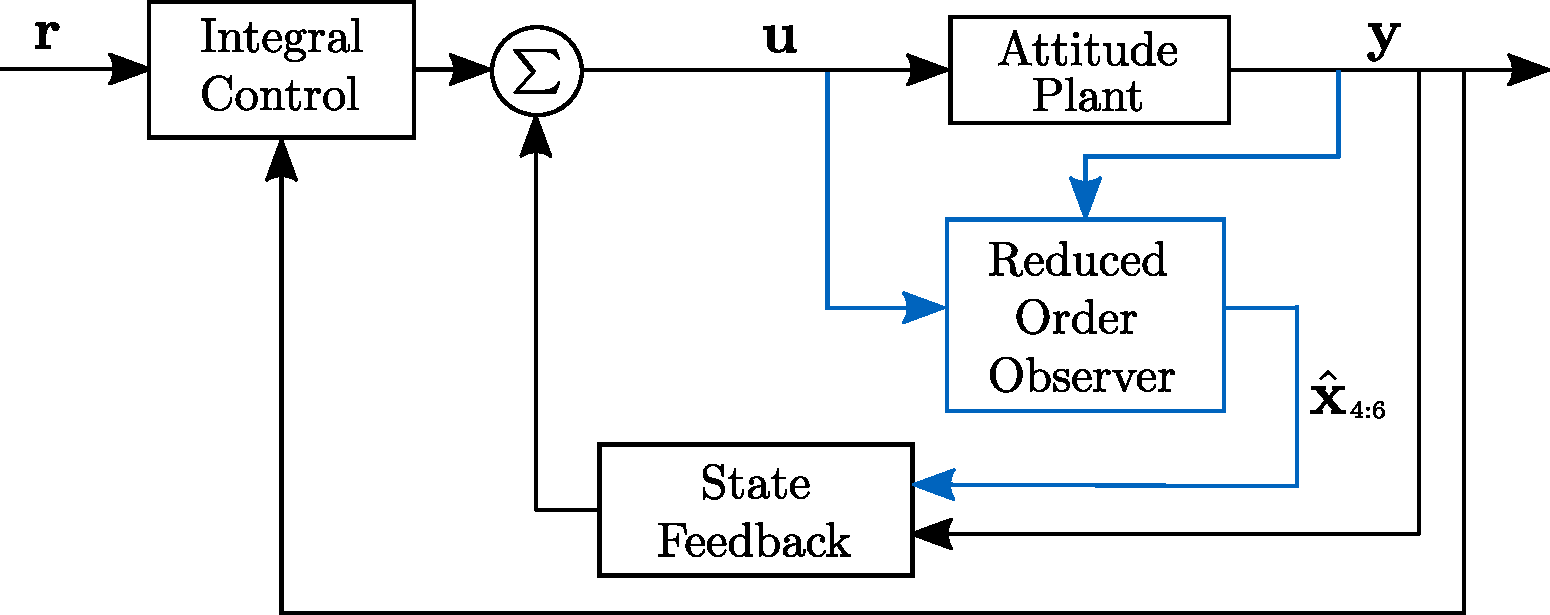
\includegraphics[width=1\textwidth]{figures/ObserverColorDiagram}
%            \end{figure}
%        \end{minipage}
%        \hspace{0.03\linewidth}
%        \begin{minipage}{0.49\linewidth}
            \begin{figure}[H]
                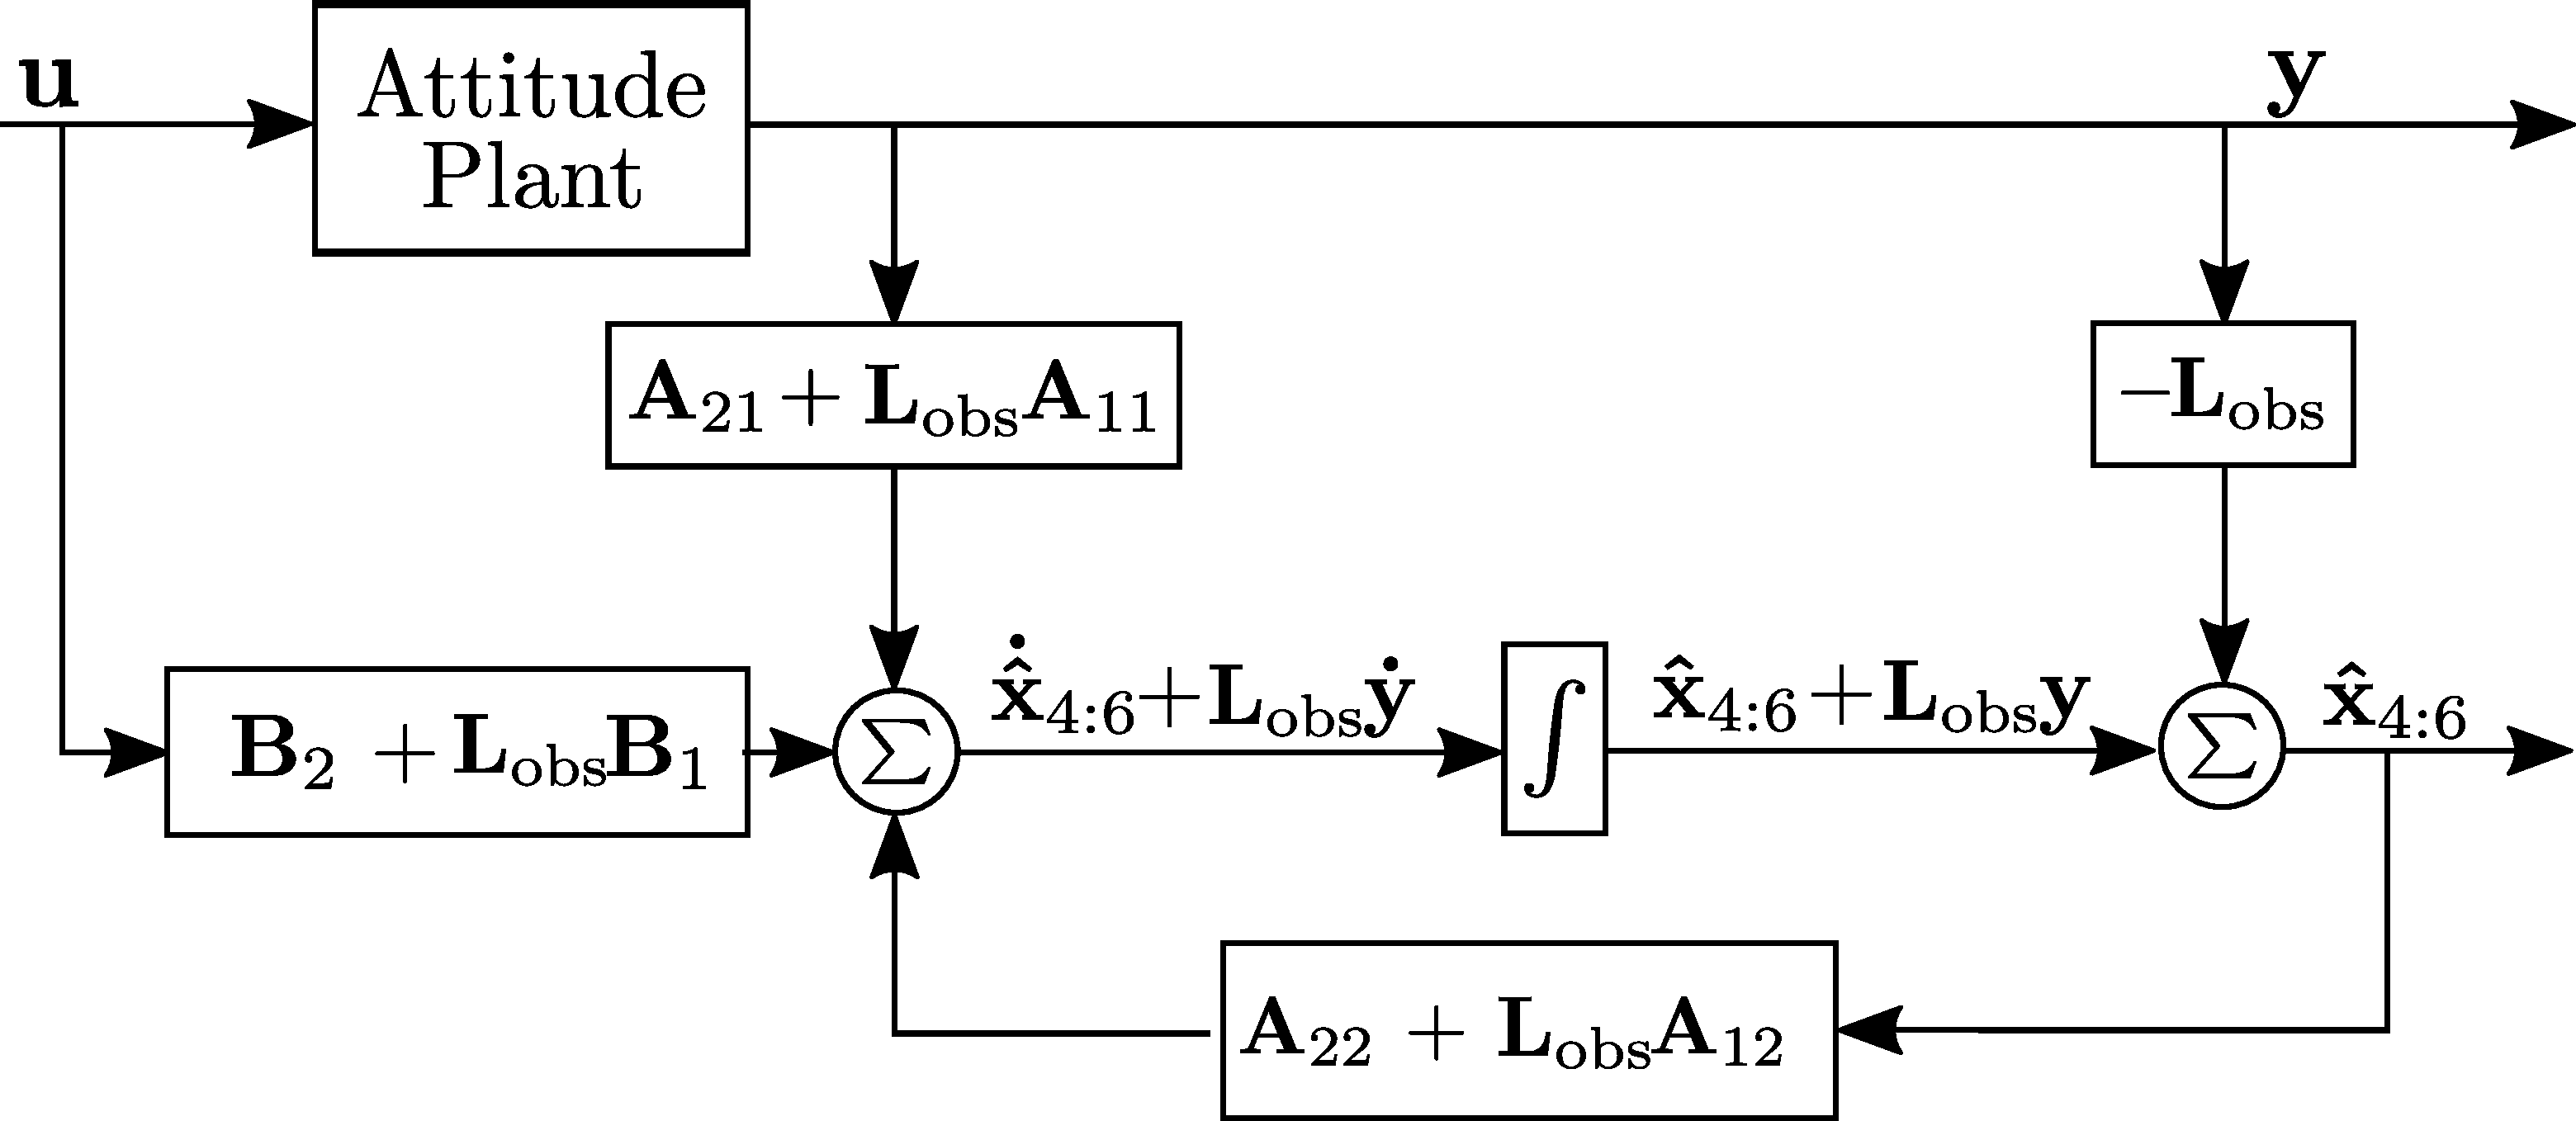
\includegraphics[width=1\textwidth]{figures/observerDiagram}
            \end{figure}                    
%        \end{minipage}
%    \end{minipage}  
    
    equation
    what are the states we estimate
   \begin{flalign}
       \vec{A_{22}} + \vec{L_{obs}}\vec{A_{12}} \nonumber
   \end{flalign}
\end{frame}

%%
% TOC
\begin{frame}{Agenda}{}
    \tableofcontents
\end{frame}

%%